\documentclass[12pt,a4paper]{article}
\usepackage{lmodern}

\usepackage{placeins}
\usepackage{amssymb,amsmath}
\usepackage{ifxetex,ifluatex}
\usepackage{fixltx2e} % provides \textsubscript
\ifnum 0\ifxetex 1\fi\ifluatex 1\fi=0 % if pdftex
  \usepackage[T1]{fontenc}
  \usepackage[utf8]{inputenc}
\else % if luatex or xelatex
  \ifxetex
    \usepackage{mathspec}
    \usepackage{xltxtra,xunicode}
  \else
    \usepackage{fontspec}
  \fi
  \defaultfontfeatures{Mapping=tex-text,Scale=MatchLowercase}
  \newcommand{\euro}{€}
\fi
% use upquote if available, for straight quotes in verbatim environments
\IfFileExists{upquote.sty}{\usepackage{upquote}}{}
% use microtype if available
\IfFileExists{microtype.sty}{%
\usepackage{microtype}
\UseMicrotypeSet[protrusion]{basicmath} % disable protrusion for tt fonts
}{}
\usepackage[lmargin = 2cm, rmargin = 2.5cm, tmargin = 2cm, bmargin = 2.5cm]{geometry}


% Figure Placement:
\usepackage{float}
\let\origfigure\figure
\let\endorigfigure\endfigure
\renewenvironment{figure}[1][2] {
    \expandafter\origfigure\expandafter[H]
} {
    \endorigfigure
}

%%%% Jens %%%%
\usepackage{titlesec}
\DeclareMathOperator*{\argmax}{arg\,max}
\DeclareMathOperator*{\argmin}{arg\,min}
\renewcommand{\vec}{\operatorname{vec}}
\newcommand{\tr}{\operatorname{tr}}
\newcommand{\Var}{\operatorname{Var}}
\newcommand{\Cov}{\operatorname{Cov}}
\newcommand{\diag}{\operatorname{diag}}

\allowdisplaybreaks

\titleformat{\section}
{\normalfont\large\bfseries}{\thesection}{1em}{}

\newcommand{\tmpsection}[1]{}
\let\tmpsection=\section
\renewcommand{\section}[1]{\tmpsection{\underline{#1}} }





%% citation setup
\usepackage{csquotes}

\usepackage[backend=biber, maxbibnames = 99, style = apa]{biblatex}
\setlength\bibitemsep{1.5\itemsep}
\addbibresource{R_packages.bib}
\usepackage{color}
\usepackage{fancyvrb}
\newcommand{\VerbBar}{|}
\newcommand{\VERB}{\Verb[commandchars=\\\{\}]}
\DefineVerbatimEnvironment{Highlighting}{Verbatim}{commandchars=\\\{\}}
% Add ',fontsize=\small' for more characters per line
\usepackage{framed}
\definecolor{shadecolor}{RGB}{248,248,248}
\newenvironment{Shaded}{\begin{snugshade}}{\end{snugshade}}
\newcommand{\AlertTok}[1]{\textcolor[rgb]{0.94,0.16,0.16}{#1}}
\newcommand{\AnnotationTok}[1]{\textcolor[rgb]{0.56,0.35,0.01}{\textbf{\textit{#1}}}}
\newcommand{\AttributeTok}[1]{\textcolor[rgb]{0.77,0.63,0.00}{#1}}
\newcommand{\BaseNTok}[1]{\textcolor[rgb]{0.00,0.00,0.81}{#1}}
\newcommand{\BuiltInTok}[1]{#1}
\newcommand{\CharTok}[1]{\textcolor[rgb]{0.31,0.60,0.02}{#1}}
\newcommand{\CommentTok}[1]{\textcolor[rgb]{0.56,0.35,0.01}{\textit{#1}}}
\newcommand{\CommentVarTok}[1]{\textcolor[rgb]{0.56,0.35,0.01}{\textbf{\textit{#1}}}}
\newcommand{\ConstantTok}[1]{\textcolor[rgb]{0.00,0.00,0.00}{#1}}
\newcommand{\ControlFlowTok}[1]{\textcolor[rgb]{0.13,0.29,0.53}{\textbf{#1}}}
\newcommand{\DataTypeTok}[1]{\textcolor[rgb]{0.13,0.29,0.53}{#1}}
\newcommand{\DecValTok}[1]{\textcolor[rgb]{0.00,0.00,0.81}{#1}}
\newcommand{\DocumentationTok}[1]{\textcolor[rgb]{0.56,0.35,0.01}{\textbf{\textit{#1}}}}
\newcommand{\ErrorTok}[1]{\textcolor[rgb]{0.64,0.00,0.00}{\textbf{#1}}}
\newcommand{\ExtensionTok}[1]{#1}
\newcommand{\FloatTok}[1]{\textcolor[rgb]{0.00,0.00,0.81}{#1}}
\newcommand{\FunctionTok}[1]{\textcolor[rgb]{0.00,0.00,0.00}{#1}}
\newcommand{\ImportTok}[1]{#1}
\newcommand{\InformationTok}[1]{\textcolor[rgb]{0.56,0.35,0.01}{\textbf{\textit{#1}}}}
\newcommand{\KeywordTok}[1]{\textcolor[rgb]{0.13,0.29,0.53}{\textbf{#1}}}
\newcommand{\NormalTok}[1]{#1}
\newcommand{\OperatorTok}[1]{\textcolor[rgb]{0.81,0.36,0.00}{\textbf{#1}}}
\newcommand{\OtherTok}[1]{\textcolor[rgb]{0.56,0.35,0.01}{#1}}
\newcommand{\PreprocessorTok}[1]{\textcolor[rgb]{0.56,0.35,0.01}{\textit{#1}}}
\newcommand{\RegionMarkerTok}[1]{#1}
\newcommand{\SpecialCharTok}[1]{\textcolor[rgb]{0.00,0.00,0.00}{#1}}
\newcommand{\SpecialStringTok}[1]{\textcolor[rgb]{0.31,0.60,0.02}{#1}}
\newcommand{\StringTok}[1]{\textcolor[rgb]{0.31,0.60,0.02}{#1}}
\newcommand{\VariableTok}[1]{\textcolor[rgb]{0.00,0.00,0.00}{#1}}
\newcommand{\VerbatimStringTok}[1]{\textcolor[rgb]{0.31,0.60,0.02}{#1}}
\newcommand{\WarningTok}[1]{\textcolor[rgb]{0.56,0.35,0.01}{\textbf{\textit{#1}}}}
\usepackage{graphicx}
\makeatletter
\def\maxwidth{\ifdim\Gin@nat@width>\linewidth\linewidth\else\Gin@nat@width\fi}
\def\maxheight{\ifdim\Gin@nat@height>\textheight\textheight\else\Gin@nat@height\fi}
\makeatother
% Scale images if necessary, so that they will not overflow the page
% margins by default, and it is still possible to overwrite the defaults
% using explicit options in \includegraphics[width, height, ...]{}
\setkeys{Gin}{width=\maxwidth,height=\maxheight,keepaspectratio}
\ifxetex
  \usepackage[setpagesize=false, % page size defined by xetex
              unicode=false, % unicode breaks when used with xetex
              xetex]{hyperref}
\else
  \usepackage[unicode=true, linktocpage = TRUE]{hyperref}
\fi
\hypersetup{breaklinks=true,
            bookmarks=true,
            pdfauthor={Dr.~Yannick Hoga},
            pdftitle={Multivariate Time Series Analysis},
            colorlinks=true,
            citecolor=black,
            urlcolor=black,
            linkcolor=black,
            pdfborder={0 0 0}}
\urlstyle{same}  % don't use monospace font for urls
\setlength{\parindent}{0pt}
\setlength{\parskip}{6pt plus 2pt minus 1pt}
\setlength{\emergencystretch}{3em}  % prevent overfull lines
\setcounter{secnumdepth}{5}

%%% Use protect on footnotes to avoid problems with footnotes in titles
\let\rmarkdownfootnote\footnote%
\def\footnote{\protect\rmarkdownfootnote}

%%% Change title format to be more compact
\usepackage{titling}

% Create subtitle command for use in maketitle
\newcommand{\subtitle}[1]{
  \posttitle{
    \begin{center}\large#1\end{center}
    }
}

\setlength{\droptitle}{-2em}
  \title{Multivariate Time Series Analysis}
  \pretitle{\vspace{\droptitle}\centering\huge}
  \posttitle{\par}
\subtitle{Solution Exercise Sheet 2}
  \author{Dr.~Yannick Hoga}
  \preauthor{\centering\large\emph}
  \postauthor{\par}
  \date{}
  \predate{}\postdate{}


%% linespread settings

\usepackage{setspace}

\onehalfspacing


% Language Setup

\usepackage{ifthen}
\usepackage{iflang}
\usepackage[super]{nth}
\usepackage[ngerman, english]{babel}

%Acronyms
\usepackage[printonlyused, withpage, nohyperlinks]{acronym}
\usepackage{changepage}

% Multicols for the Title page
\usepackage{multicol}


% foot


\begin{document}

\selectlanguage{english}

%%%%%%%%%%%%%% Jens %%%%%
\numberwithin{equation}{section}




\restoregeometry


%%% Header 

\begin{minipage}{0.6\textwidth}
University of Duisburg-Essen\\
Faculty of Business Administration and Economics\\
Chair of Econometrics\\
\end{minipage}

%\begin{minipage}{0.4\textwidth}
	\begin{flushright}
	\vspace{-3cm}
	\includegraphics*[width=5cm]{Includes/duelogo_en.png}\\
	\vspace{.125cm}
	\end{flushright}
%\end{minipage}
%\vspace{.125cm}
\hspace{-0.005cm}Winter Term 2019/2020

\vspace{0.05cm}

\begin{center}
	\vspace{.25cm}
	Dr.~Yannick Hoga \hspace{.5cm} Thilo Reinschlüssel \\
	\vspace{.25cm}
	\textbf{\Large{Multivariate Time Series Analysis}}\\
	\vspace{.25cm}
	\textbf{\large{Solution Exercise Sheet 2}}\\
	\vspace{.125cm}
\end{center}




% body from markdown

\hypertarget{exercise-1-moments-and-simulation-of-a-var1-process}{%
\section{Exercise 1: Moments and Simulation of a VAR(1)
Process}\label{exercise-1-moments-and-simulation-of-a-var1-process}}

Take the model from Example 2.4 on Slide 2-6:

\begin{itemize}
  \item[a)] Derive a formula to obtain the population cross-covariance matrices for the lags $1$ to $10$ and compute them using R.
  \item[] \textit{Hint: A glance at the slides might save you some time.}
\end{itemize}

\emph{Solution:}

\begin{align*}
  z_t & = \phi_1 z_{t-1} + a_t\\
  \\
  \Gamma_0 & = E \left( z_t - \mu  \right) \left( z_t - \mu  \right)^{'}\\
  & = E \left[ \phi_1 \left( z_{t -1} - \mu \right) \left( z_{t -1} - \mu \right)^{'} \phi_1^{'} \right] + E \left[a_t a_t^{'} \right]\\
    & =\phi_1  \ \Gamma_0 \ \phi_1^{'} + \Sigma_a\\
  \Leftrightarrow \vec(\Gamma_0) &= (\phi_1 \otimes \phi_1) \cdot \vec(\Gamma_0) + \vec(\Sigma_a) \\
  \Leftrightarrow \vec(\Gamma_0) &= (I_{K^2} - \phi_1 \otimes \phi_1) \cdot \vec(\Sigma_a) \\
 \Rrightarrow \Gamma_1 & = \phi_1 \Gamma_0\\
 \Rrightarrow \Gamma_l & = \phi_{l-1} \Gamma_{l-1} = \phi_1^{l} \Gamma_0\\
\end{align*}

\begin{itemize}
  \item[b)] Based on your results, compute the cross-correlation matrices.
  \item[] \textit{Hint: A loop might save you some time.}
\end{itemize}

\emph{Solution:}

\begin{Shaded}
\begin{Highlighting}[]
\CommentTok{# First define parameters/coefficients:}
\NormalTok{Phi <-}\StringTok{ }\KeywordTok{matrix}\NormalTok{(}\DataTypeTok{data =} \KeywordTok{c}\NormalTok{(}\FloatTok{0.8}\NormalTok{, }\FloatTok{-0.3}\NormalTok{, }\FloatTok{0.4}\NormalTok{, }\FloatTok{0.6}\NormalTok{), }
              \DataTypeTok{byrow =} \OtherTok{FALSE}\NormalTok{, }\DataTypeTok{nrow =} \DecValTok{2}\NormalTok{) }\CommentTok{# VAR coefficients}

\NormalTok{Sigma_a <-}\StringTok{ }\KeywordTok{matrix}\NormalTok{(}\DataTypeTok{data =} \KeywordTok{c}\NormalTok{(}\DecValTok{2}\NormalTok{, }\FloatTok{0.5}\NormalTok{, }\FloatTok{0.5}\NormalTok{, }\FloatTok{1.0}\NormalTok{), }
                  \DataTypeTok{byrow =} \OtherTok{FALSE}\NormalTok{, }\DataTypeTok{nrow =} \DecValTok{2}\NormalTok{) }\CommentTok{# innovations' covariances}

\NormalTok{Phi_kron <-}\StringTok{ }\KeywordTok{kronecker}\NormalTok{(}\DataTypeTok{X =}\NormalTok{ Phi, }\DataTypeTok{Y =}\NormalTok{ Phi) }\CommentTok{# kronecker product}
 \CommentTok{# alternative command: Phi %x% Phi}

\NormalTok{Ident <-}\StringTok{ }\KeywordTok{diag}\NormalTok{(}\KeywordTok{ncol}\NormalTok{(Phi_kron)) }
\CommentTok{# identity matrix with the same dimensions as Phi_kron}

\NormalTok{Gamma0.vec <-}\StringTok{ }\KeywordTok{solve}\NormalTok{(Ident }\OperatorTok{-}\StringTok{ }\NormalTok{Phi_kron) }\OperatorTok\StringTok{ }\KeywordTok{c}\NormalTok{(Sigma_a) }
\CommentTok{# c() works like the "vec" operator}

\NormalTok{Gamma0.mat <-}\StringTok{ }\KeywordTok{matrix}\NormalTok{(}\DataTypeTok{data =}\NormalTok{ Gamma0.vec, }\DataTypeTok{nrow =} \DecValTok{2}\NormalTok{, }\DataTypeTok{byrow =} \OtherTok{FALSE}\NormalTok{)}

\NormalTok{mat_names <-}\StringTok{ }\KeywordTok{c}\NormalTok{(}\StringTok{'z_1'}\NormalTok{, }\StringTok{'z_2'}\NormalTok{) }\CommentTok{# setting names of the series}
\KeywordTok{colnames}\NormalTok{(Gamma0.mat) <-}\StringTok{ }\NormalTok{mat_names }\CommentTok{# passing column names}
\KeywordTok{rownames}\NormalTok{(Gamma0.mat) <-}\StringTok{ }\NormalTok{mat_names }\CommentTok{# assig row names}
\end{Highlighting}
\end{Shaded}

The \(\Gamma_0\) matrix is then:

\begin{verbatim}
##           z_1   z_2
## z_1  5.933333 -0.45
## z_2 -0.450000  2.65
\end{verbatim}

To derive the \(\Gamma_1\) matrix, we can simply apply the following
formula.

\begin{align*}
  \Gamma_1 & = \phi_1 \Gamma_0\\
\end{align*}

\begin{Shaded}
\begin{Highlighting}[]
\NormalTok{Gamma1.mat <-}\StringTok{ }\NormalTok{Phi }\OperatorTok\StringTok{ }\NormalTok{Gamma0.mat}
\end{Highlighting}
\end{Shaded}

\(\Gamma_1\) is then:

\begin{verbatim}
##           z_1   z_2
## z_1  4.566667 0.700
## z_2 -2.050000 1.725
\end{verbatim}

To derive all \(l^{th}\) lagged covariance matrices we can use the more
general equation and program a loop over all desired lags.

\begin{align*}
  \Rrightarrow \Gamma_l & = \phi_{l-1} \Gamma_{l-1} = \phi_1^{l} \Gamma_0\\
\end{align*}

To derive the correlation matrices \(\rho_l\) we divide the covariances
by the standard deviations.

\begin{align*}
 \rho_l & = \left( \rho_{ij} (l)\right)_{i,j = 1}^{K} = D^{-1} \Gamma_l D^{-1}  \\
 \\
   & = 
  \begin{pmatrix}
    \dfrac{\Cov(x_t , x_{t-l})}{\sqrt{\Var(x_t) \cdot \Var(x_{t- l})}} &
    \dfrac{\Cov(x_t , y_{t-l})}{\sqrt{\Var(x_t) \cdot \Var(y_{t- l})}}\\
    \dfrac{\Cov(y_t , x_{t-l})}{\sqrt{\Var(y_t) \cdot \Var(x_{t- l})}} &
    \dfrac{\Cov(y_t , y_{t-l})}{\sqrt{\Var(y_t) \cdot \Var(y_{t- l})}}
  \end{pmatrix}\\
\end{align*}

\begin{itemize}
  \item where $D  = \diag \left\{ \sqrt{\Gamma_{11} (0)}, \ldots , \sqrt{\Gamma_{kk} (0)} \right\}$ 
\end{itemize}

\begin{Shaded}
\begin{Highlighting}[]
\CommentTok{# compute further (lagged) cross-covariance-functions}
\CommentTok{# preparing the variables to store the matrices into }
\CommentTok{#covariance}
\NormalTok{ccovf.list <-}\StringTok{ }\KeywordTok{list}\NormalTok{() }
\CommentTok{#correlation}
\NormalTok{ccorf.list <-}\StringTok{ }\KeywordTok{list}\NormalTok{() }

\CommentTok{# obtaining standard deviations for the single variables (parts of z) }
\CommentTok{# and putting them in a diagonal matrix}
\NormalTok{D.inv <-}\StringTok{ }\KeywordTok{solve}\NormalTok{(}\KeywordTok{sqrt}\NormalTok{(Gamma0.mat }\OperatorTok{*}\StringTok{ }\KeywordTok{diag}\NormalTok{(}\KeywordTok{ncol}\NormalTok{(Phi)))) }

\ControlFlowTok{for}\NormalTok{ (i }\ControlFlowTok{in} \DecValTok{1}\OperatorTok{:}\DecValTok{10}\NormalTok{)\{}
    
    \CommentTok{# covariance}
\NormalTok{    ccovf <-}\StringTok{ }\NormalTok{Phi}\OperatorTok\NormalTok{i }\OperatorTok\StringTok{ }\NormalTok{Gamma0.mat}
    \KeywordTok{rownames}\NormalTok{(ccovf) <-}\StringTok{ }\NormalTok{mat_names}
\NormalTok{  ccovf.list[[i]] <-}\StringTok{ }\NormalTok{ccovf}
    
    \CommentTok{# correlation}
\NormalTok{    ccorf <-}\StringTok{  }\NormalTok{D.inv }\OperatorTok\StringTok{ }\NormalTok{ccovf.list[[i]] }\OperatorTok\StringTok{ }\NormalTok{D.inv}
    \KeywordTok{rownames}\NormalTok{(ccorf) <-}\StringTok{ }\NormalTok{mat_names}
\NormalTok{  ccorf.list[[i]] <-}\StringTok{ }\NormalTok{ccorf}
\NormalTok{\}}
\NormalTok{ccovf.list }\CommentTok{# cross lagged covariances}
\end{Highlighting}
\end{Shaded}

\begin{verbatim}
## [[1]]
##           z_1   z_2
## z_1  4.566667 0.700
## z_2 -2.050000 1.725
## 
## [[2]]
##           z_1   z_2
## z_1  2.833333 1.250
## z_2 -2.600000 0.825
## 
## [[3]]
##           z_1  z_2
## z_1  1.226667 1.33
## z_2 -2.410000 0.12
## 
## [[4]]
##             z_1    z_2
## z_1  0.01733333  1.112
## z_2 -1.81400000 -0.327
## 
## [[5]]
##            z_1     z_2
## z_1 -0.7117333  0.7588
## z_2 -1.0936000 -0.5298
## 
## [[6]]
##           z_1      z_2
## z_1 -1.006827  0.39512
## z_2 -0.442640 -0.54552
## 
## [[7]]
##            z_1       z_2
## z_1 -0.9825173  0.097888
## z_2  0.0364640 -0.445848
## 
## [[8]]
##            z_1        z_2
## z_1 -0.7714283 -0.1000288
## z_2  0.3166336 -0.2968752
## 
## [[9]]
##            z_1        z_2
## z_1 -0.4904892 -0.1987731
## z_2  0.4214086 -0.1481165
## 
## [[10]]
##            z_1         z_2
## z_1 -0.2238279 -0.21826509
## z_2  0.3999919 -0.02923795
\end{verbatim}

\begin{Shaded}
\begin{Highlighting}[]
\NormalTok{ccorf.list }\CommentTok{# cross lagged correlations}
\end{Highlighting}
\end{Shaded}

\begin{verbatim}
## [[1]]
##            z_1       z_2
## z_1  0.7696629 0.1765329
## z_2 -0.5169893 0.6509434
## 
## [[2]]
##            z_1       z_2
## z_1  0.4775281 0.3152374
## z_2 -0.6556937 0.3113208
## 
## [[3]]
##            z_1        z_2
## z_1  0.2067416 0.33541257
## z_2 -0.6077777 0.04528302
## 
## [[4]]
##              z_1        z_2
## z_1  0.002921348  0.2804352
## z_2 -0.457472478 -0.1233962
## 
## [[5]]
##            z_1        z_2
## z_1 -0.1199551  0.1913617
## z_2 -0.2757949 -0.1999245
## 
## [[6]]
##            z_1         z_2
## z_1 -0.1696899  0.09964527
## z_2 -0.1116293 -0.20585660
## 
## [[7]]
##              z_1         z_2
## z_1 -0.165592809  0.02468636
## z_2  0.009195853 -0.16824453
## 
## [[8]]
##            z_1         z_2
## z_1 -0.1300160 -0.02522625
## z_2  0.0798518 -0.11202838
## 
## [[9]]
##             z_1         z_2
## z_1 -0.08266671 -0.05012857
## z_2  0.10627500 -0.05589301
## 
## [[10]]
##            z_1         z_2
## z_1 -0.0377238 -0.05504425
## z_2  0.1008739 -0.01103319
\end{verbatim}

\begin{itemize}
  \item[c)] Draw a corresponding innovation sequence $a_t$ for 300 periods from a (multivariate) Gaussian distribution and simulate the given VAR(1) process without any further built-in functions.
  \item[] \textit{Hint: 'mvrnorm' and 'for' are still allowed}
\end{itemize}

\emph{Solution:}\\

\begin{itemize}
  \item Steps:
  \begin{enumerate}
    \item Set $T$ (in code $N$)
    \item Draw $\left\{ a_1, \ldots , a_T \right\} \sim \left[ \mu , \Sigma_a \right]$
    \item Set $z_0 = \mathbb{E} \left( z_t\right)$
    \item $z_1 = \phi_1 z_0 + a_1$
    \item Repeat Step 4 $(T - 1)$ times
    \item (Discard the first few observations to minimize effects of $z_0$ on the results)
    \begin{itemize}
      \item[$\Rightarrow$] \textit{Note} that it is generally advised to discard the first few observations to eliminate the influence of the arbitrary starting point! In our case we skipped this step to keep things short and clear.
    \end{itemize}
  \end{enumerate}
\end{itemize}

\begin{Shaded}
\begin{Highlighting}[]
\CommentTok{# i) Set sample size and further coefficients}
\NormalTok{N <-}\StringTok{ }\DecValTok{300}
\CommentTok{# ii) The Basis: Innovations}
\KeywordTok{set.seed}\NormalTok{(}\DecValTok{2}\OperatorTok{^}\DecValTok{9-1}\NormalTok{) }\CommentTok{# for replication: the 'random' numbers drawn }
\CommentTok{# up from this point will always be the same (given you use }
\CommentTok{# the same command to draw them...)}
\NormalTok{a <-}\StringTok{ }\KeywordTok{mvrnorm}\NormalTok{(}\DataTypeTok{n =}\NormalTok{ N, }\DataTypeTok{mu =} \KeywordTok{c}\NormalTok{(}\DecValTok{0}\NormalTok{,}\DecValTok{0}\NormalTok{), }\DataTypeTok{Sigma =}\NormalTok{ Sigma_a)}
\CommentTok{# iii) Writing a function to generate 'z' realisations from 'a' using Phi}
\NormalTok{var1gen <-}\StringTok{ }\ControlFlowTok{function}\NormalTok{(coef.mat, z.lag, innovation)\{}
\NormalTok{  z.current <-}\StringTok{ }\NormalTok{coef.mat }\OperatorTok\StringTok{ }\NormalTok{z.lag }\OperatorTok{+}\StringTok{ }\NormalTok{innovation }
  \CommentTok{# z_(t) = phi * z_(t-1) + a_(t)}
  \KeywordTok{return}\NormalTok{(z.current)}
\NormalTok{\}}
\CommentTok{# iv) Prepare variable for 'z'}
\NormalTok{z <-}\StringTok{ }\KeywordTok{ts}\NormalTok{(}\DataTypeTok{data =} \KeywordTok{matrix}\NormalTok{(}\DataTypeTok{data =} \OtherTok{NA}\NormalTok{, }\DataTypeTok{nrow =}\NormalTok{ (N), }\DataTypeTok{ncol =} \KeywordTok{ncol}\NormalTok{(Phi))}
\NormalTok{        ,}\DataTypeTok{start =} \DecValTok{1}\NormalTok{, }\DataTypeTok{names =}\NormalTok{ mat_names)}
\CommentTok{# v) Set starting values for z (at mean + innovation)}
\NormalTok{z[}\DecValTok{1}\NormalTok{,] <-}\StringTok{ }\KeywordTok{c}\NormalTok{(}\DecValTok{0}\NormalTok{,}\DecValTok{0}\NormalTok{) }\OperatorTok{+}\StringTok{ }\NormalTok{a[}\DecValTok{1}\NormalTok{,]}
\CommentTok{# vi) Generate z repeatedly and store it}
\ControlFlowTok{for}\NormalTok{ (i }\ControlFlowTok{in} \DecValTok{2}\OperatorTok{:}\NormalTok{(N))\{}
\NormalTok{  z[i,] <-}\StringTok{ }\KeywordTok{var1gen}\NormalTok{(}\DataTypeTok{coef.mat =}\NormalTok{ Phi, }\DataTypeTok{z.lag =}\NormalTok{ z[(i}\DecValTok{-1}\NormalTok{),], }\DataTypeTok{innovation =}\NormalTok{ a[i,])}
\NormalTok{\}}
\end{Highlighting}
\end{Shaded}

\begin{itemize}
  \item[d)] Plot the multivariate time series you have just created. Does it look stationary?
\end{itemize}

\emph{Solution:}\\

The ordinary organic \texttt{plot} command works because \(z\) is
already a \emph{ts}-class object (among other classes) and not a data
frame.

\begin{Shaded}
\begin{Highlighting}[]
\KeywordTok{plot}\NormalTok{(z)}
\end{Highlighting}
\end{Shaded}

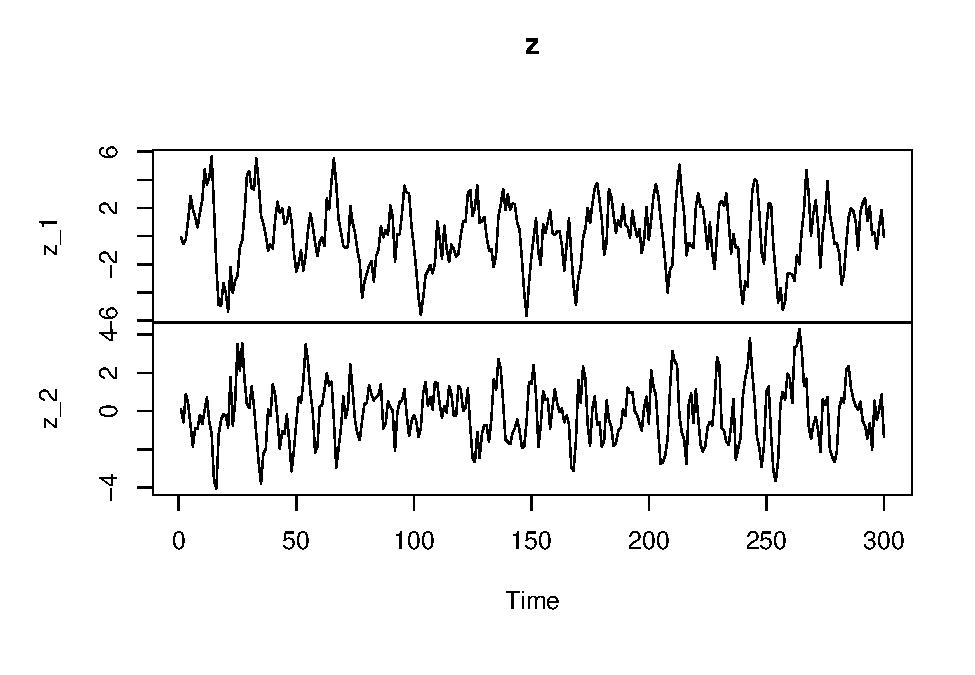
\includegraphics{solution_exercise_2_files/figure-latex/unnamed-chunk-7-1.pdf}

At least it looks stable hence we cannot rule out stationarity.

\begin{itemize}
  \item[e)] Estimate the sample cross-covariance and cross-correlation matrices. Compare these with the population moment matrices from task a)
\end{itemize}

\emph{Solution:}

\begin{align*}
  \widehat{\Gamma_0} & = \tilde{z}_T^{'} \tilde{z}_{T-1} \cdot (T - 1)^{-1} \\
  \tilde{z}_T^{'} & = z_T - \widehat{\mu}_z\\
  Z & \ \text{is a} \ T \times 2 \ \text{matrix}\\
  z_t &\  \text{is a} \ 2 \times 1 \ \text{vector}\\
  z_t & := 
  \begin{pmatrix}
    x_t \\
    y_t
  \end{pmatrix} \; \leftarrow \text{variables}\\
  Z_t & := 
  \begin{pmatrix}
    X_{t} & Y_{t} \\
    X_{t-1} & Y_{t-1} \\
    X_{t-2} & Y_{t-2} \\
    \vdots & \vdots \\
    X_{t-t} & Y_{t-t} \\
  \end{pmatrix} \; \leftarrow \text{sample data}\\
  \widehat{\Cov(x_t, y_{t-1})} & = \dfrac{1}{(T - 1)} \sum_{t = 1}^{T}  \left( \tilde{X}_t \cdot \tilde{Y}_{t- 1} \right)\\
  \Rightarrow & \ \text{is part of:} \dfrac{1}{T -1} \cdot \tilde{Z}_t^{'} \tilde{Z}_{t-1} = \widehat{\Gamma_1}
\end{align*}

To estimate moments from simulated data one can simply use the command
\texttt{cov()} respectively \texttt{cor()} , but we do it by
\enquote{hand} to get a thorough understanding and see the relation to
the Yule-Walker equation.

First we need to demean the multivariate time series. Therefore, we
calculate the column means.

\begin{Shaded}
\begin{Highlighting}[]
\NormalTok{mu <-}\StringTok{ }\KeywordTok{colMeans}\NormalTok{(z)}
\end{Highlighting}
\end{Shaded}

To demean the series we now have two coding options to proceed with, one
would be to iterate over the rows and subtracte the mean vector every
time.

\begin{Shaded}
\begin{Highlighting}[]
\NormalTok{z.demeaned <-}\StringTok{ }\KeywordTok{t}\NormalTok{(}\KeywordTok{apply}\NormalTok{(}\DataTypeTok{X =}\NormalTok{ z, }\DataTypeTok{MARGIN =} \KeywordTok{c}\NormalTok{(}\DecValTok{1}\NormalTok{), }\DataTypeTok{FUN =} \ControlFlowTok{function}\NormalTok{(x) x }\OperatorTok{-}\StringTok{ }\NormalTok{mu))}
\end{Highlighting}
\end{Shaded}

The other option would be to subtracte the column means from each column
individually.

\begin{Shaded}
\begin{Highlighting}[]
\NormalTok{z.demeaned <-}\StringTok{ }\KeywordTok{cbind}\NormalTok{(z[,}\DecValTok{1}\NormalTok{]}\OperatorTok{-}\NormalTok{mu[}\DecValTok{1}\NormalTok{], z[,}\DecValTok{2}\NormalTok{]}\OperatorTok{-}\NormalTok{mu[}\DecValTok{2}\NormalTok{])}
\end{Highlighting}
\end{Shaded}

Now we are able to compute \(\widehat{\Gamma_0}\).

\begin{Shaded}
\begin{Highlighting}[]
\NormalTok{Gamma0.hat <-}\StringTok{ }\KeywordTok{t}\NormalTok{(z.demeaned) }\OperatorTok\StringTok{ }\NormalTok{z.demeaned }\OperatorTok{/}\StringTok{ }\NormalTok{(N}\DecValTok{-1}\NormalTok{) }
\end{Highlighting}
\end{Shaded}

Since we already demeaned the series we need to correct the degrees of
freedom \((N - 1)\). Please also note that now the first entry is
transposed! ( \emph{z.demeaned} is a data matrix and not a random vector
anymore!)

To compute \(\widehat{\rho}_0\) we just need to standardize
\(\widehat{\Gamma}_0\).

\begin{Shaded}
\begin{Highlighting}[]
\NormalTok{standardisation <-}\StringTok{ }\KeywordTok{matrix}\NormalTok{(}\DataTypeTok{data =} \KeywordTok{c}\NormalTok{(Gamma0.hat[}\DecValTok{1}\NormalTok{,}\DecValTok{1}\NormalTok{], }
                                   \KeywordTok{sqrt}\NormalTok{( Gamma0.hat[}\DecValTok{1}\NormalTok{,}\DecValTok{1}\NormalTok{] }\OperatorTok{*}\StringTok{ }\NormalTok{Gamma0.hat[}\DecValTok{2}\NormalTok{,}\DecValTok{2}\NormalTok{]),}
                                   \KeywordTok{sqrt}\NormalTok{(Gamma0.hat[}\DecValTok{2}\NormalTok{,}\DecValTok{2}\NormalTok{] }\OperatorTok{*}\StringTok{ }\NormalTok{Gamma0.hat[}\DecValTok{1}\NormalTok{,}\DecValTok{1}\NormalTok{]),}
\NormalTok{                                   Gamma0.hat[}\DecValTok{2}\NormalTok{,}\DecValTok{2}\NormalTok{]),}
                       \DataTypeTok{nrow =} \DecValTok{2}\NormalTok{, }\DataTypeTok{byrow =} \OtherTok{FALSE}\NormalTok{) }
\NormalTok{Rho0.hat <-}\StringTok{ }\NormalTok{Gamma0.hat }\OperatorTok{/}\StringTok{ }\NormalTok{standardisation}
\end{Highlighting}
\end{Shaded}

This is just another way to program it, maybe it makes it more visible
what is inside \(D.inv \ \%*\% \ D.inv\) (from the lecture slides).

Then \(\widehat{\rho_0}\) is:

\begin{verbatim}
##             z_1         z_2
## z_1  1.00000000 -0.04910251
## z_2 -0.04910251  1.00000000
\end{verbatim}

Since we simulated the trajectory with the \enquote{true} values we can
compare the estimations with these values. The estimated mean values for
the two series are slightly negative \((0.1762664, -0.1272957 )^{'}\) so
the differences are also slightly negative since we simulated the time
series without a mean \(\mu_{1,2} = 0\).

For the covariance \(\Gamma_0\) we calculated the analytical solution in
part \emph{b} of this exercise. The differences
\((\widehat{\Gamma}_0 - \Gamma_0)\) are:

\begin{verbatim}
##            z_1        z_2
## z_1 -0.5964760  0.2778575
## z_2  0.2778575 -0.3470556
\end{verbatim}

The same applies for the comparison of the correlations \(\rho_0\) and
the estimated correlations \(\widehat{\rho_0}\). The differences
\((\widehat{\rho}_0 - \rho_0 )\) are:

\begin{verbatim}
##            z_1          z_2
## z_1 0.00000000 6.438295e-02
## z_2 0.06438295 2.220446e-16
\end{verbatim}

\hypertarget{exercise-2-checking-var1-stationarity}{%
\section{Exercise 2: Checking VAR(1)
Stationarity}\label{exercise-2-checking-var1-stationarity}}

Recall the conditions to check if a VAR(1) process is stationary. Now
assume the VAR(1) model \(z_{t} = \phi_{1} z_{t-1} + a_{t}\) with
\(a_{t}\) as a sequence of i.i.d. innovations:

\begin{itemize}
\item[a)] Do you need to make further assumptions on the cross-correlations of $a_{t}$ to ensure stationarity?
\end{itemize}

\emph{Solution:}

\begin{align*}
  Z_t & = \phi_1 Z_{t-1} + a_t\\
  a_t & \overset{i.i.d.}{\sim} \left[ \mu_a , \Sigma_a \right]\\
  i.i.d.: & \Cov (a_t , a_{t-1}) = 0
\end{align*}

Generally not, since i.i.d. errors induce no dynamic structure. Still,
finite \(1^{st}\) and \(2^{nd}\) moments are required for weak
stationarity! (Gaussian innovations fulfill that condition, of course).

\begin{itemize}
 \item[b)] Which of the following processes are stationary? $\phi_{1} = \dots $ \\
\begin{itemize} 
    \item[i)] $ \begin{pmatrix}
    0.2 & 0.3 \\ 
    -0.6 & 1.1
    \end{pmatrix} $
    \hspace{8em}
    \item[ii)] $ \begin{pmatrix}
    0.5 & 0.3 \\ 
    0 & -0.3
    \end{pmatrix} $
    %\hspace{8em}
    \item[iii)] $ \begin{pmatrix}
    1 & 0 \\ 
    0 & 1
    \end{pmatrix} $
    \hspace{8em}
    \item[iv)] $ \begin{pmatrix}
    1 & -1 \\ 
    1 & -1
    \end{pmatrix} $
    \hspace{8em}
    \item[v)] $ \begin{pmatrix}
    1 & -0.5 \\ 
    -0.5 & 0
    \end{pmatrix} $
\end{itemize}
\end{itemize}

\emph{Solution:}

\begin{align*}
  Z_t & = \phi_1 z_{t-1} + a_t\\
  & = \phi_1 \cdot(\phi_1 z_{t-2} + a_{t-1}) + a_t \\
    & = \underbrace{ \phi_1^p \ z_{t-p}}_{\text{stable ?}} + \underbrace{\sum_{i = 0}^{p} \phi_1^{i} \ a_{t -1} }_{\text{summable ?}}
\end{align*} \begin{align*}
  & \lim_{p \rightarrow \infty} \phi_1^p \longrightarrow 0_{k \times k} \\
  & \Rightarrow \text{eigenvalues !} \\
  & \Rightarrow \phi_1 x = \lambda x \Rightarrow \phi_1^{p} x = \lambda^p x\\
  & \Rightarrow \text{solve:} \left( \phi_1 - I_K \lambda \right) x = 0\\
  & \text{for} \ x \neq 0: \left| \phi_1 - I_K \lambda \right| \overset{!}{=} 0 \\
  & \text{stability (for stationarity)}  \left| \lambda_1 \right|, \ldots,  \left| \lambda_k \right| < 1 \\
\end{align*}

\begin{itemize} 
    \item[i)] $\begin{pmatrix}
        0.2 & 0.3 \\ 
        -0.6 & 1.1 \\
      \end{pmatrix} $
\end{itemize}

\begin{align*}
   = & \begin{pmatrix}
        0.2 & 0.3 \\ 
        -0.6 & 1.1 \\
      \end{pmatrix} - 
      \begin{pmatrix}
       \lambda & 0 \\ 
       0 & \lambda
      \end{pmatrix}\\
      = &  
      \left|
      \begin{matrix}
      (0.2 - \lambda) & 0.3 \\ 
        -0.6 & (1.1 - \lambda)
      \end{matrix}
      \right| \\
      = & (0.2 -\lambda)(1.1 - \lambda) - (-0.6) (0.3)\\
      = & \lambda^2 - 1.3 \lambda + 0.4 \overset{!}{=} 0 \\
      pq \text{-formula} \Rightarrow  \lambda_{1,2} = & - \left( \dfrac{-1.3}{2} \right) \pm \sqrt{ \left( \dfrac{-1.3}{2} \right)^2 - 0.4 }\\
       = & 0.65 \pm 0.15 \\
      \lambda_1 = & 0.8 \\
      \lambda_2 = & 0.5 \\
      & |\lambda_1| < 1 , |\lambda_2| < 1,  \; \text{stationary}
\end{align*}

\begin{itemize} 
    \item[ii)] $ \begin{pmatrix}
    0.5 & 0.3 \\ 
    0 & -0.3
    \end{pmatrix} $
\end{itemize}

\begin{align*}
  & \left|
  \begin{matrix}
    0.5 - \lambda & 0.3 \\ 
    0 &  -0.3 - \lambda
    \end{matrix}
    \right| \\
    = & (0.5 - \lambda)(-0.3 - \lambda) - 0.3 \cdot 0 \overset{!}{=} 0 \\
    \Rightarrow & \lambda_1 = 0.5, \; \lambda_2 = 0.3 \Rightarrow \text{stationary} 
\end{align*}

\begin{itemize}     
        \item[iii)] $ \begin{pmatrix}
    1 & 0 \\ 
    0 & 1
    \end{pmatrix} $
\end{itemize}

\begin{align*}
  & \left|
  \begin{matrix}
    1 - \lambda & 0 \\ 
    0 &  1 - \lambda
    \end{matrix}
    \right| \\
    = & (1 - \lambda)(1 - \lambda) - 0 \cdot 0 \overset{!}{=} 0 \\
    \Rightarrow & \lambda_1 = 1, \; \lambda_2 = 1 \Rightarrow \text{not stationary} 
\end{align*}

\begin{itemize}
    \item[iv)] $ \begin{pmatrix}
    1 & -1 \\ 
    1 & -1
    \end{pmatrix} $
\end{itemize}

\begin{align*}
  & \left|
  \begin{matrix}
    1 - \lambda & -1 \\ 
    1 &  -1 - \lambda
    \end{matrix}
    \right| \\
    = & (1 - \lambda)(-1 - \lambda) - 0 \cdot 0 \overset{!}{=} 0 \\
    = & \lambda^2 + \lambda - \lambda - 1 +1 \\
    = & \lambda^2 \overset{!}{=} 0\\
    \Rightarrow & \lambda_1 = 0, \; \lambda_2 = 0 \Rightarrow \text{ stationary} 
\end{align*}

\begin{itemize}
    \item[v)] $ \begin{pmatrix}
    1 & -0.5 \\ 
    -0.5 & 0
    \end{pmatrix} $
\end{itemize}

\begin{align*}
  & \left|
  \begin{matrix}
    1 - \lambda & -0.5 \\ 
    -0.5 &  0 - \lambda
    \end{matrix}
    \right| \\
    = & (1 - \lambda)( - \lambda) - 0.5 \cdot 0.5 \overset{!}{=} 0 \\
    = & \lambda^2 - \lambda - 0.25 \overset{!}{=} 0\\
    \Rightarrow & \lambda_1 = 0.207, \; \lambda_2 = 1.207 \Rightarrow \text{not stationary} 
\end{align*}

\end{document}
